%----------------------------------------------------------------------------------------
%	PACKAGES AND THEMES
%----------------------------------------------------------------------------------------
\documentclass[aspectratio=169,xcolor=dvipsnames]{beamer}
\usetheme{SimplePlusAIC}

\usepackage{hyperref}
\usepackage{graphicx} % Allows including images
\usepackage{booktabs} % Allows the use of \toprule, \midrule and  \bottomrule in tables
\usepackage{svg} %allows using svg figures
\usepackage{tikz}
\usepackage{makecell}
\newcommand*{\defeq}{\stackrel{\text{def}}{=}}
\usepackage{comment}
\usepackage{bm}



\usepackage{mathtools}

\NewDocumentCommand{\expect}{ e{^} s o >{\SplitArgument{1}{||}}m }{%
	\operatorname{\mathbb{E}}%     the expectation operator
	\IfValueT{#1}{{\!}^{#1}}% the measure of the expectation
	\IfBooleanTF{#2}{% *-variant
		\expectarg*{\expectvar#4}%
	}{% no *-variant
		\IfNoValueTF{#3}{% no optional argument
			\expectarg{\expectvar#4}%
		}{% optional argument
			\expectarg[#3]{\expectvar#4}%
		}%
	}%
}
\NewDocumentCommand{\expectvar}{mm}{%
	#1\IfValueT{#2}{\nonscript\;\delimsize\vert\nonscript\;#2}%
}
\DeclarePairedDelimiterX{\expectarg}[1]{[}{]}{#1}

%Select the Epilogue font (requires luaLatex or XeLaTex compilers)
\usepackage{fontspec}
\setsansfont{Epilogue}[
    Path=./epilogueFont/,
    Scale=0.8,
    Extension = .ttf,
    UprightFont=*-Regular,
    BoldFont=*-Bold,
    ItalicFont=*-Italic,
    BoldItalicFont=*-BoldItalic
    ]
    
    \newcommand{\bbR}{\mathbb{R}}
    \newcommand{\bfX}{\mathbf{X}}
    \newcommand{\bfAlp}{\bm{\alpha}}
    \renewcommand\qedsymbol{$\blacksquare$}
    \newcommand{\dpartial}[2]{\frac{\partial #1}{\partial #2}}
    \newcommand{\norm}[1]{\left\lVert#1\right\rVert}
    \DeclareMathOperator{\Tr}{Tr}
    \DeclareMathOperator*{\argmin}{arg\,min}
    
    

    %\usepackage[sorting=none,style=numeric]{biblatex}
    %\addbibresource{references.bib}
    \usepackage[style=authoryear]{biblatex}
    \addbibresource{references.bib}
    
%----------------------------------------------------------------------------------------
%	TITLE PAGE
%----------------------------------------------------------------------------------------

\title[Deep learning for high dimensional PDE's]{Deep learning methods for high dimensional partial differential equations} % The short title appears at the bottom of every slide, the full title is only on the title page
\subtitle{An application to control problems}

\author[Contreras]{Carlos Daniel Contreras Quiroz}
\institute[U. Andes]{Tesis de maestría \newline Departamento de matemáticas \newline Universidad de los Andes}
% Your institution as it will appear on the bottom of every slide, maybe shorthand to save space


\date{30 de Junio 2023} % Date, can be changed to a custom date
%----------------------------------------------------------------------------------------
%	PRESENTATION SLIDES
%----------------------------------------------------------------------------------------

\begin{document}

\begin{frame}[plain]
    % Print the title page as the first slide
    \titlepage
\end{frame}

\begin{comment}
	\begin{frame}{Contenido}
		% Throughout your presentation, if you choose to use \section{} and \subsection{} commands, these will automatically be printed on this slide as an overview of your presentation
		\tableofcontents
	\end{frame}
	
\end{comment}

%------------------------------------------------
\section{Motivación}
%------------------------------------------------

\begin{frame}{Motivación}
Las ecuaciones en derivadas parciales son útiles para modelar todo tipo de fenómenos
\begin{enumerate}
	\item En finanzas la ecuación de Black-Scholes
\begin{equation}
	\frac{\partial V}{\partial t}+\frac{1}{2} \sigma^2 S^2 \frac{\partial^2 V}{\partial S^2}+r S \frac{\partial V}{\partial S}-r V=0
\end{equation}
\item En control estocástico la ecuación HJB \begin{equation}
	\begin{split}
		&\dpartial{V}{t}+H(t,x,D_x V,D_{xx} V)=0\\
		&V(T,x)=g(x),
	\end{split}
\end{equation}
\item En mecánica cuántica la ecuación de Schrödinger \begin{equation}
	i \hbar \frac{\partial}{\partial t} \Psi(x, t)=\left[-\frac{\hbar^2}{2 m} \frac{\partial^2}{\partial x^2}+V(x, t)\right] \Psi(x, t)
\end{equation}
\end{enumerate}
\end{frame}

\begin{frame}{Motivación: La maldición de la dimensionalidad}
Usualmente no tenemos acceso a soluciones analíticas, por lo cual usamos métodos numéricos como
\begin{enumerate}
	\item Diferencias finitas
	\item Elementos finitos
	\item Métodos espectrales
\end{enumerate}
Todos estos sufren la "\textit{la maldición de la dimensionalidad}" ("\textit{the curse of dimensionality}"). Esto es, la complejidad computacional incrementa exponencialmente con la dimensión del problema que se quiere resolver $O(N^d)$.
\end{frame}

\begin{frame}{Motivación: La maldición de la dimensionalidad}
	Pero hay problemas interesantes en dimensiones altas
	\begin{enumerate}
		\item Evaluar el precio justo de una opción que tiene muchos activos subyacentes
		\item Encontrar controles óptimos para problemas con espacio de estados grande
		\item Encontrar la dinámica cuántica de un problema de muchos cuerpos para diseñar chips o nuevos fármacos
	\end{enumerate}
Entonces ¡necesitamos métodos para resolverlas!
\end{frame}
%------------------------------------------------
\begin{frame}{La nueva idea}
	Un problema similar surge en la modelación estadística de datos, para lo cual se han propuesto técnicas de \textit{machine learning}. En particular, el uso de \textit{redes neuronales artificiales}(ANN) ha mostrado ser útil para resolver cierto tipo de problemas.\\
	\vspace*{5mm}
	Queremos usar estas mismas herramientas para resolver este problema para ecuaciones en derivadas parciales
\end{frame}

\begin{frame}{¿Qué es una red neuronal?}
    \begin{columns}[c] % The "c" option specifies centered vertical alignment while the "t" option is used for top vertical alignment
	
	\column{.6\textwidth} % Left column and width
\begin{figure}
	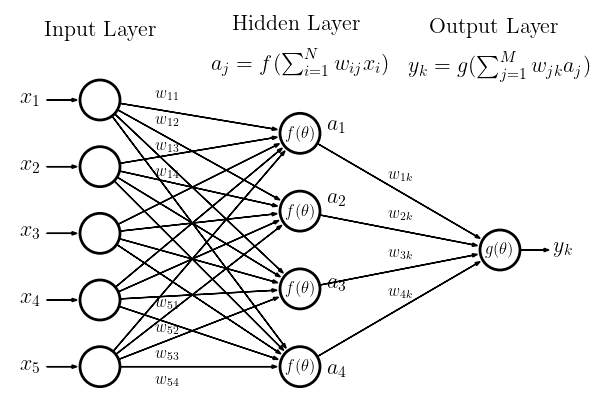
\includegraphics[width=\linewidth]{images/neural_net.png}
\end{figure}
	
	\column{.35\textwidth} % Right column and width
Son una forma \textbf{expresiva} de parametrizar funciones $\varphi_\theta:\bbR^n\to \bbR^m$, mediante composición de operaciones sencillas
\begin{equation*}
	x_{k+1}=\sigma(Wx_k+b)
\end{equation*}
Y podemos calcular $\nabla_\theta \varphi$ usando la regla de la cadena: diferenciación automática(AD).
\end{columns}
\end{frame}
\begin{frame}{Varias perspectivas}
	La idea es usar este tipo de parametrizaciones para resolver PDE's. Para esto se han planteado varias formas
	\begin{enumerate}
		\item Deep Galerkin Method (DGM) y Physics Informed Neural Networks(PINNs)
		\item Fourier Neural Operators
		\item \textbf{Métodos basados en BSDEs} 
	\end{enumerate}
\end{frame}

\begin{comment}
	    \begin{block}{Block}
		Sample text
	\end{block}
	
	\begin{alertblock}{Alertblock}
		Sample text in red box
	\end{alertblock}
	
	\begin{examples}
		Sample text in green box. The title of the block is ``Examples".
	\end{examples}
\end{comment}

\begin{frame}{¿Que es una BSDE?}
	Una SDE standard en $[0,T]$ es de la forma
	\begin{equation}
		\label{eqn:SDE}
		\begin{split}
			X_t&=x_0+\int_0^t b\left(s, X_s\right) d s+\int_0^t \sigma\left(s, X_s\right) d W_s\\
			X_0&=x_0,
		\end{split}
	\end{equation}
¿Qué pasa si la consideramos hacia atrás, con una condición terminal? 

\begin{equation}
	\begin{split}
	X_t&=\xi+\int_t^T b\left(s, X_s\right) d s+\int_t^T \sigma\left(s, X_s\right) d W_s\\
	X(T)&=\xi
\end{split}
\end{equation}
Nada asegura que $X_t$ sea $\mathcal{F}_t$-medible, por lo que el problema no está bien puesto.
\end{frame}
\begin{frame}{¿Que es una BSDE?}
	Podemos forzar este proceso para ser $\mathcal{F}_t$-medible añadiendo un proceso $Z$ que le "restará" estocásticidad a $\xi$ para que la solución sea adaptada.   
	\begin{equation}
		Y_t=\xi+\int_t^T b\left(s, Y_s, Z_s\right) d s-\int_t^T Z_s d W_s
	\end{equation}
Que se puede escribir hacia adelante como 
\begin{equation}
\label{eqn:BSDE}
\begin{split}
	&dY_t=-f(t,Y_t,Z_t)dt+Z_t\cdot dW_t\\
	&Y(T)=\xi
\end{split}
\end{equation}
Noten el cambio de notación $X_t:=Y_t$ y $b:=f$
\end{frame}

\begin{frame}{FBSDE}
	También podemos acoplar una SDE con una BSDE para obtener una ecuación Forward-Backward .
	\begin{equation}
		\label{eqn:FBSDE}
		\begin{split}
			&dX_s=\mu(t,X_s)ds+\sigma(s,X_s)dW_s\\
			&X_t=x\\
			&dY_s=-f(s,X_s,Y_s,Z_s)ds+Z_s dW_s\\
			&Y_T=g(X_T),
		\end{split}
	\end{equation}
\end{frame}

\begin{frame}{Relación con PDEs}
	Lo importante de estos procesos es que los podemos relacionar con ecuaciones en derivadas parciales de la forma
	\begin{equation}
		\label{eqn:FKNolineal}
		\begin{split}
			&\dpartial{u}{t}(t,x)+\mathcal{L}_t u(t,x)+f(t,x,u(t,x),\sigma(t,x)' D_x u(t,x))=0\\
			&u(T,x)=g(x),
		\end{split}
	\end{equation} 
donde 

\begin{equation}
	\label{eqn:ininitesimalGen}
		\mathcal{L}_tv=\mu(t,x)\cdot D_x u(t,x)+\frac{1}{2}\Tr(\sigma(t,x)\sigma'(t,x)D_{xx}^2u(t,x))
\end{equation} 
es el generador del proceso $X_t$.
\end{frame}

\begin{frame}{Relación con PDEs}
	Podemos asociar la solución $(X_t,Y_t,Z_t)$ de una FBSDE con una PDE de en la forma anterior mediante el siguiente teorema
	\begin{theorem}[\cite{pham_continuous-time_2009}]
		Bajo \textit{ciertas} hipótesis de regularidad, si $v$ es una solución clásica de \eqref{eqn:FKNolineal} entonces los procesos $dX_t=\mu(t,X_t)dt+\sigma(t,X_t)\cdot dW_t\quad X(0)=x $ $Y_t=u(t,X_t)$ y $ Z_t=\sigma(t,X_t)' D_x u(t,X_t)$ son solución de la FBSDE \eqref{eqn:FBSDE}.\\
		\vspace*{5mm}
		Recíprocamente, si $(X_t,Y_t,Z_t)$ es una solución de \eqref{eqn:FBSDE}, entonces $u(t,x)=Y^{t,x}_{t}$ es continua y es una solución viscosa a (\ref{eqn:FKNolineal}). 
	\end{theorem}
\end{frame}
	

\begin{frame}{El método Deep BSDE }
Vamos a explotar esta conexión para resolver la PDE usando simulaciones de la FBSDE de la siguiente forma \parencite{han_solving_2018}
\begin{itemize}

	\item Discretizamos la FBSDE usando el esquema de Euler-Maruyama
	\begin{equation}
		\label{eqn:EMForward}
		X_{t_{n+1}} \approx X_{t_n} +\mu\left(t_n, X_{t_n}\right) \Delta t_n+\sigma\left(t_n, X_{t_n}\right) \Delta W_{t_n}
	\end{equation}
y
\begin{equation}
	\label{eqn:EMBackward}
	\begin{aligned}
		u\left(t_{n+1}, X_{t_{n+1}}\right)
		&\approx  u\left(t_n, X_{t_n}\right) -f\left(t_n, X_{t_n}, u\left(t_n, X_{t_n}\right), \sigma'\left(t_n, X_{t_n}\right) D_x u\left(t_n, X_{t_n}\right)\right) \Delta t_n \\
		& +\sigma\left(t_n, X_{t_n}\right)'D_x u\left(t_n, X_{t_n}\right)  \Delta W_{t_n},
	\end{aligned}
\end{equation}
	\item Parametrizamos la funciones $X_0 \to u(0,Y_0)$ y $X_t\to \sigma'(t,X_t)D_x u(t,X_t)$ con redes neuronales 
\item Optimizamos los parámetros de la red intentando llegar a la condición terminal usando el costo
\begin{equation}
	\label{eqn:lossDeepBSDE}
	\ell(\theta)=\expect*{|g(X_{t_N})-\hat{u}(\{X_{t_n}\}_{0}^N,\{W_{t_n}\}_{0}^N)|^2},
\end{equation}

\end{itemize}
\end{frame}

\begin{frame}{El método Deep BSDE}
	\begin{figure}
		\centering
		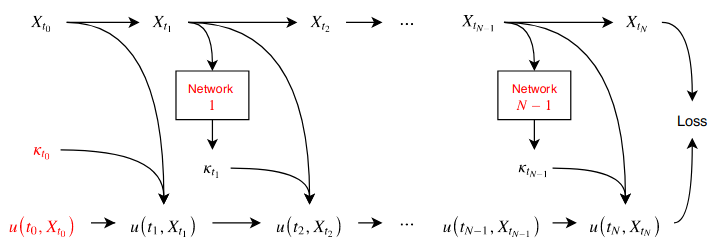
\includegraphics[width=\linewidth]{images/DeepBSDEMap}
		\label{fig:deepbsdemap}
	\end{figure}
\end{frame}

\begin{frame}{Estructura de la red}
	La estructura y método de optimización de la red que escojamos influye mucho en la calidad de la aproximación y velocidad de convergencia. En el articulo original se usó
	\begin{itemize}
		\item Una red completamente acoplada con 2 capas intermedias y d+10 neuronas en cada capa
		\item La función de activación $ReLu$
		\item Capas intermedias de normalización
		\item Recorte de gradientes 
		\item El método ADAM para optimizar la red
	\end{itemize}
\end{frame}

\begin{frame}{Variantes: Merged Deep BSDE}
	Desde entonces se han planteado varias variantes de este método
	\begin{itemize}
		\item Merged Deep BSDE \parencite{chan-wai-nam_machine_2018}: Aproximar el gradiente con una sola red neuronal que incluya el tiempo en sus entradas
		\begin{figure}
			\centering
			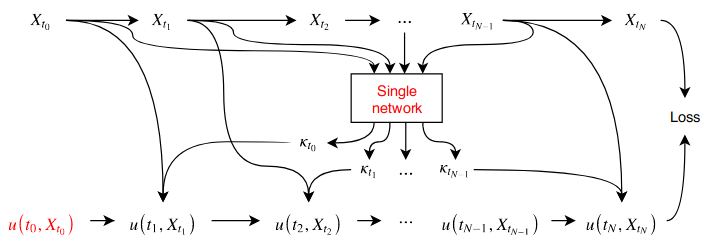
\includegraphics[width=\linewidth]{images/MergedBSDE}
			\label{fig:mergedbsde}
		\end{figure}
	\end{itemize}
\end{frame}

\begin{frame}{Variantes: Merged Residual BSDE}
		\begin{itemize}
		\item Merged Residual Deep BSDE \parencite{chan-wai-nam_machine_2018}: Aproximar el gradiente con una sola red neuronal que incluya el tiempo en sus entradas y usar una arquitectura con shortcuts
		\begin{figure}
			\centering
			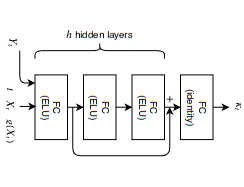
\includegraphics[width=0.6\linewidth,height=5cm]{images/Residual.png}
			\label{fig:residualmergedstructure}
		\end{figure}
	\end{itemize}
\end{frame}

\begin{frame}{Variantes: Método de Raissi}
	\begin{itemize}
		\item Raissi's method\parencite{raissi_forward-backward_2018}: Aproximar directamente la solución de la PDE con una red neuronal, calcular las derivadas espaciales con diferenciación automática y optimizar la red con un costo que modele la diferencias locales de la evolución temporal  
	\begin{equation}
		\begin{gathered}
			\ell(\theta):=\mathbb{E}\left[\sum_{i=0}^{N-1} \Phi\left(t_i, X_{t_i}, Y_{t_i}, Y_{t_{i+1}}, \Delta W_{t_{i}}\right)+\left(g\left(X_{t_N}\right)-Y_{t_N}\right)^2\right] \\
		\end{gathered}
	\end{equation}
	donde
	\begin{equation}
		\begin{split}
			\Phi\left(t_i, X_{t_i}, Y_{t_i}, Y_{t_{i+1}}, \Delta W_{t_i}\right)&=\left(Y_{t_{i+1}}-Y_{t_i}+f\left(t_i, X_{t_i}, Y_{t_i}, \sigma'\left(t_i, X_{t_i}\right) \widehat{Z}_{t_i}\right)\left(\Delta t_i\right)\right. \\
			&\left.-\widehat{Z}_{t_i}' \sigma\left(t_i, X_{t_i}\right)\left(\Delta W_{t_i}\right)\right)^2,
		\end{split}
	\end{equation}
	\end{itemize}
\end{frame}

\begin{frame}{Ejemplo: Control estocástico}
	Supongamos que tenemos 3 partículas en $\bbR^2$ cuyo estado conjunto describimos con un vector $\vec{X}=(x_1,y_1,x_2,y_2,x_3,y_3)\in \bbR^6$, que se mueven satisfaciendo la dinámica
	\begin{equation}
		\begin{split}
			&dX_t=2\sqrt{\lambda}\alpha_t dt+\sqrt{2\nu}dW_t\\
			&X_0=x_0.
		\end{split} 
	\end{equation} 
	Queremos elegir el control $\alpha_t$ para llevar a todas las partículas hacia un punto dado usando la menor cantidad de combustible posible y evitando que estén cerca entre sí.
\end{frame}

\begin{frame}{Ejemplo: Control estocástico}
	Esto es, queremos elegir el control $\alpha_t$ que minimiza el costo dado por 
	\begin{equation}
		J(\alpha_t)=\mathbb{E}\left[\int_{0}^{T}(|\alpha_t|^2+F(t,X_t)) dt +g(X_T)\right],
	\end{equation}   
	donde modelamos la aversión entre partículas con
	\begin{equation}
		F(t,X_t)=F(t,(\vec{x}_1,\vec{x}_2,\vec{x}_3))=C\left(e^{-\frac{|\vec{x}_1-\vec{x}_2|^2}{\sigma}}+e^{-\frac{|\vec{x}_1-\vec{x}_3|^2}{\sigma}}+e^{-\frac{|\vec{x}_2-\vec{x}_3|^2}{\sigma}}\right),
	\end{equation}
	y su deseo para llegar al estado terminal $z_T$ por 
\begin{equation}
	g(x)=|x-z_T|^2.
\end{equation}
¿Cómo elegimos el mejor control?
\end{frame}

\begin{frame}{Programación dinámica: Ecuación HJB}
	Definimos el costo empezando en un estado $x$ y tiempo $t$ usando el control $\alpha$ como
	\begin{equation}
		J(t,x,\alpha)=\mathbb{E}\left[\int_{t}^{T}f(s,X_s^{t,x,\alpha},\alpha_s) ds +g(X_T^{t,x,\alpha})\right].
	\end{equation}
Y la función de valor como
\begin{equation}
	V(t,x)=\sup_{\alpha\in\mathcal{A}[t,T]}J(t,x,\alpha).
\end{equation}
Entonces, del principio de programación dinámica se establece que esta debe cumplir la ecuación de Hamilton-Jacobi-Bellman 
\begin{equation}
	\begin{split}
		&\dpartial{V}{t}+\inf_{a\in A}\{\mathcal{L}^a[V](t,x)+f(t,x,a)\}=0\\
		&V(T,x)=g(x),
	\end{split}
\end{equation}
\end{frame}

\begin{frame}{Ejemplo: Control estocástico}
	En este caso la ecuación a resolver es 
	\begin{equation}
		\label{eqn:HJB_example}
		\dpartial{V}{t}+\nu \Delta V -\lambda |\nabla V|^2+F(t,x)=0,
	\end{equation}
sujeto a la condición terminal
\begin{equation}
	V(T,x)=g(x).
\end{equation}
Si la resolvemos, podemos acceder a controles óptimos a través de $\hat{\alpha}(t,x)=-\sqrt{\lambda}D_x V(t,x)$. \\

\vspace*{5mm}
Sin embargo, esta ecuación es no lineal y está definida en $\bbR^6$, por lo que no podemos usar métodos como diferencias finitas. Por otro lado, existe una representación probabilística de la solución
\begin{equation}
	\label{eqn:probabilisticExact}
	V(t,x)=-\frac{\nu}{\lambda}\ln\left(\expect*{\exp \left(-\frac{\lambda}{\nu} g(x+\sqrt{2\nu}W_{T-t})-\frac{\lambda}{\nu}\int_{t}^{T}F(s,x+\sqrt{2\nu}W_{s-t})ds\right)}\right).
\end{equation}
\end{frame}

\begin{frame}{Ejemplo: Control estocástico}
	Usemos el método Deep BSDE. En este marco el proceso hacia adelante tendría drift y volatilidad dadas por
\begin{equation}
	\mu(t,x)=0\quad \quad \sigma(t,x)=\sqrt{2\nu} \mathbb{I}_{6\times 6}
\end{equation}
y la parte no lineal es 
\begin{equation}
	f(t,x,V(t,x),\sigma(t,x)'D_x V(t,x))=-\lambda |D_x V|^2+F(t,x).
\end{equation}
\end{frame}

\begin{frame}{Resultados}
	    \begin{columns}[c] % The "c" option specifies centered vertical alignment while the "t" option is used for top vertical alignment
		
		\column{.45\textwidth} % Left column and width
\begin{figure}
	\centering
	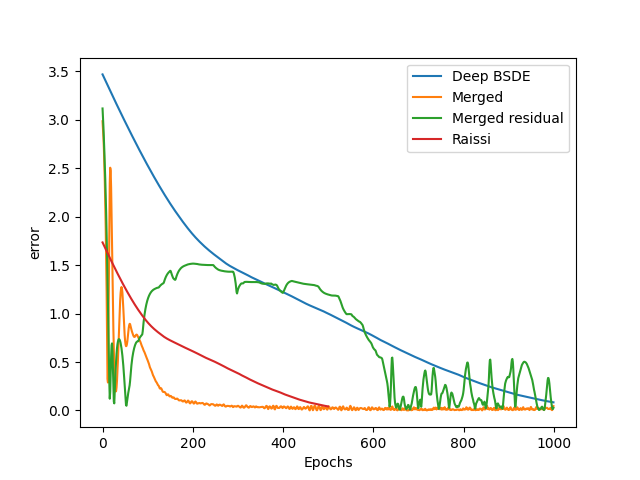
\includegraphics[width=1.1\linewidth]{images/training}
	\caption{Curvas de entrenamiento}
	\label{fig:training}
\end{figure}
		\column{.5\textwidth} % Right column and width
		\vspace*{4mm}
\begin{figure}
	\centering
	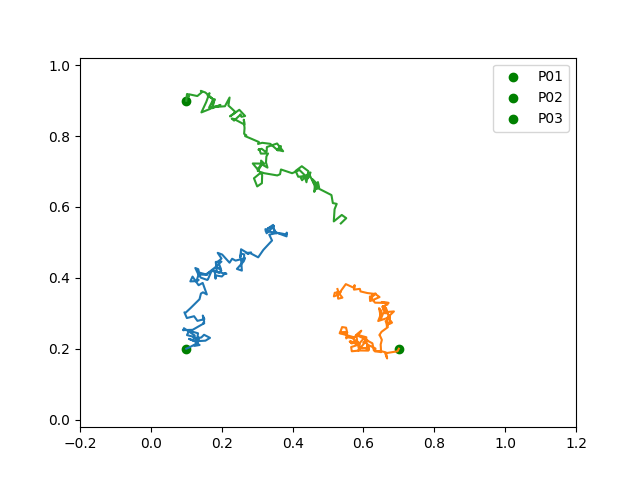
\includegraphics[width=\linewidth]{images/OptimalLQRCentrilized}
	\caption{Ejemplo de trayectoria óptima }
	\label{fig:optimallqrcentrilized}
\end{figure}
\end{columns}
\end{frame}

\begin{frame}{Problemas acotados}
Ahora, consideremos problemas en dominio acotados $\Omega$ 
	\begin{equation}
		\label{eqn:FKNolinealBoun}
		\begin{split}
			&\dpartial{u}{t}(t,x)+\mathcal{L}_t u(t,x)+f(t,x,u(t,x),\sigma(t,x)' D_x u(t,x))=0\\
			&u(T,x)=g(x),
		\end{split}
	\end{equation} 
con condiciones de frontera de Dirichlet y Neumann
\begin{align}
	&u(t,x)=h_d(x) \quad \forall x\in \Gamma_D \quad \forall t\in[0,T] \label{eqn:DirichletBoundary}\\
	&\dpartial{u}{n}(t,x)=h_n(x) \quad \forall x\in \Gamma_N \quad \forall t\in[0,T] \label{eqn:NeumanBoundary},
\end{align}
\end{frame}

\begin{frame}{Deep Galerkin Method}
	Una forma muy general de resolver PDE's es forzando todo en el costo de la red. Esto se conoce como el método de Deep Galerkin o Physics Informed Neural Networks \parencite{sirignano_dgm_2018}. En este caso, aproximamos la solución $v$ con una red neuronal $\varphi$ y la entrenamos con el costo
	\begin{equation}
		\label{eqn:DGMLoss}
		\begin{split}
			\mathcal{L}(\varphi):=&\alpha_{int}\mathcal{L}_{\text{DGM,int}}(\varphi)+\alpha_{T}\mathcal{L}_{\text{DGM,T}}(\varphi)+\alpha_{d}\mathcal{L}_{\text{DGM,d}}(\varphi)+\alpha_{n}\mathcal{L}_{\text{DGM,n}}(\varphi) \\
			:=&\alpha_{int}\norm{\dpartial{\varphi}{t}+\mathcal{L}\varphi+f(t,x,\varphi(t,x),\sigma(t,x)'D_x \varphi(t,x))}_{[0,T]\times \Omega,\nu_1}^2\\
			+&\alpha_{T}\norm{\varphi(T,x)-g(x)}_{\Omega,\nu_2}^2\\
			+&\alpha_{d}\norm{\varphi(t,x)-h_d(x)}_{[0,T]\times \partial \Gamma_D,\nu_3 }^2\\
			+&\alpha_{n}\norm{\hat{n}\cdot D_x \varphi(t,x)-h_n(x)}_{[0,T]\times \partial \Gamma_N,\nu_4 }^2
		\end{split},
	\end{equation}
donde todas las derivadas se calculan con diferenciación automática.
\end{frame}

\begin{frame}{Interpolación Deep BSDE-PINNS}
	Podemos combinarlo con el método Deep BSDE usando el \textbf{costo de difusión} \parencite{nusken_interpolating_2023}
	\begin{equation}
		\mathcal{L}_{\text {diff }}^{\mathrm{t}}(\varphi)=\alpha_{\text {int }} \mathcal{L}_{\text {diff,int }}^{\mathrm{t}}(\varphi)+\alpha_{\mathrm{T}} \mathcal{L}_{\text {diff, } \mathrm{T}}^{\mathrm{t}}(\varphi)+\alpha_{\mathrm{d}} \mathcal{L}_{\text {diff, } \mathrm{d}}^{\mathrm{t}}(\varphi)+\alpha_{\mathrm{n}} \mathcal{L}_{\text {diff, } \mathrm{n}}^{\mathrm{t}}(\varphi)
	\end{equation}
donde
\begin{equation}
	\begin{aligned}
		& \mathcal{L}_{\text {diff,int }}^{\mathrm{t}}(\varphi)=\mathbb{E}\left[\left(\varphi\left(\mathcal{T},X_{\mathcal{T}} \right)-\varphi\left(t_0,X_{t_0}\right)-\int_{t_0}^{\mathcal{T}} \sigma^{\top} \nabla \varphi\left(s,X_s\right) \cdot \mathrm{d} W_s\right.\right. \\
		& \left.\left.+\int_{t_0}^{\mathcal{T}} f\left(s,X_s, \varphi\left(s,X_s\right), \sigma^{\top} \nabla \varphi\left(s,X_s\right)\right) \mathrm{d} s\right)^2\right] \text {, } \\
		 &\mathcal{L}_{\text {diff,T }}^{\mathrm{t}}(\varphi)=\mathbb{E}\left[\left(\varphi\left(T,X^{(T)}\right)-g\left(X^{(T)}\right)\right)^2\right] ,
		 \mathcal{L}_{\text {diff, } \mathrm{d}}^{\mathrm{t}}(\varphi)=\mathbb{E}\left[\left(\varphi\left(t^{\mathrm{d}},X^{\mathrm{d}}\right)-h_d\left(t^{\mathrm{d}},X^{\mathrm{d}}\right)\right)^2\right], \\
		&
		\mathcal{L}_{\text {diff, } \mathrm{n}}^{\mathrm{t}}(\varphi)=\mathbb{E}\left[\left(D_x\varphi\left(t^{\mathrm{n}},X^{\mathrm{n}} \right)-h_n\left(t^{\mathrm{n}},X^{\mathrm{n}}\right)\right)^2\right]. \\
	\end{aligned}
\end{equation}
\end{frame}

\begin{frame}{Ejemplo: Control estocástico}
	Este problema modela una partícula que quiere salir de una habitación por la puerta 
	\begin{figure}
		\centering
		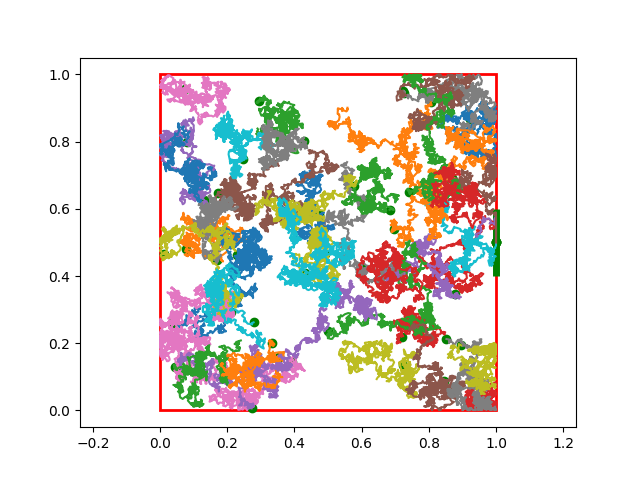
\includegraphics[height=6cm]{images/pathsInterp}
		\label{fig:pathsinterp}
	\end{figure}
\end{frame}

\begin{frame}{Ejemplo: Control estocástico}
	Consideremos un caso de control LQR con ecuación HJB
	\begin{equation}
		\label{eqn:HJB2D}
		\dpartial{V}{t}+\nu \Delta V -\lambda |\nabla V|^2+1=0,
	\end{equation} 
	sujeto a las condiciones de Diriclet y Neumann
	\begin{equation}
		V(t,x)=0 \quad \text{ for } x\in \partial\Omega_d, 
	\end{equation}
	\begin{equation}
		\dpartial{V}{\vec{n}}(t,x)=0 \quad \text{ for } x\in \partial\Omega_n, 
	\end{equation}
	con condición terminal
	\begin{equation}
		V(1.0,x)=0 \quad \text{ for } x\in \Omega.
	\end{equation}
\end{frame}



\begin{frame}{Resultados}
		    \begin{columns}[c] % The "c" option specifies centered vertical alignment while the "t" option is used for top vertical alignment
		
		\column{.45\textwidth} % Left column and width
		\begin{figure}
			\centering
			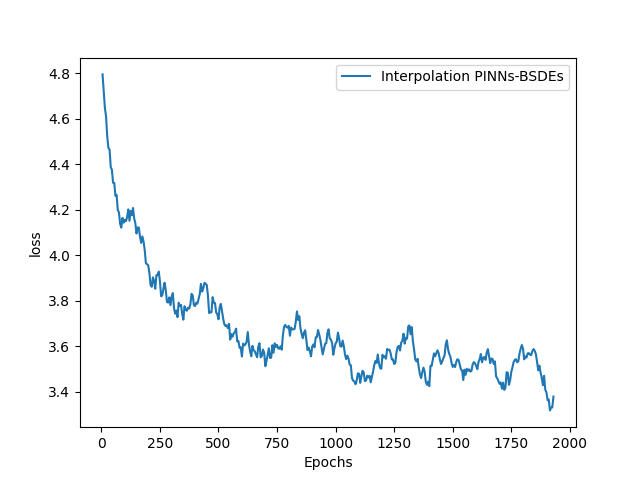
\includegraphics[width=\linewidth]{images/Interp_training.png}
			\caption{Curva de entrenamiento Interpolación}
		\end{figure}
		
		\column{.5\textwidth} % Right column and width
		\vspace*{4mm}
		\begin{figure}
			\centering
			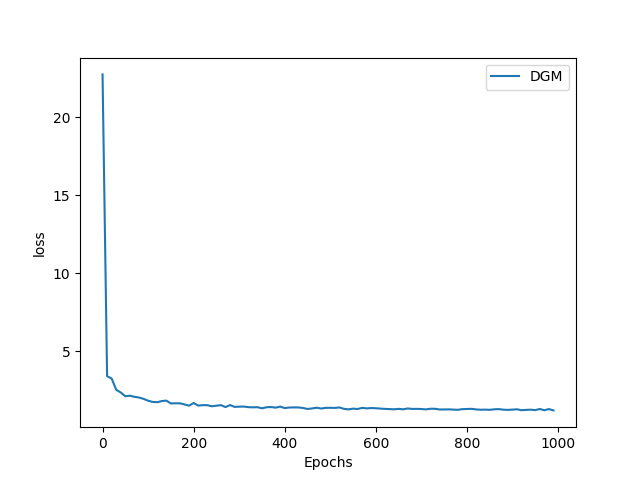
\includegraphics[width=\linewidth]{images/trainingDGM.png}
			\caption{Curva de entrenamiento DGM}
		\end{figure}
	\end{columns}
\end{frame}

\begin{frame}{Resultados}
	\begin{columns}[c] % The "c" option specifies centered vertical alignment while the "t" option is used for top vertical alignment
		
		\column{.45\textwidth} % Left column and width
		\begin{figure}
			\centering
			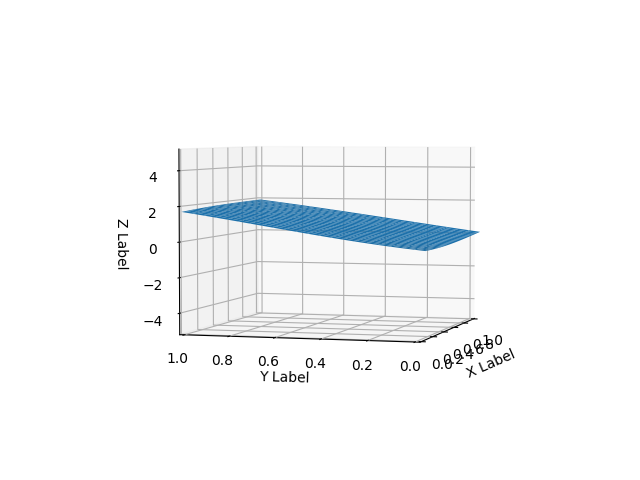
\includegraphics[width=\linewidth]{images/Sol_DGM.png}
		\end{figure}
		
		\column{.5\textwidth} % Right column and width
		\vspace*{4mm}
		\begin{figure}
			\centering
			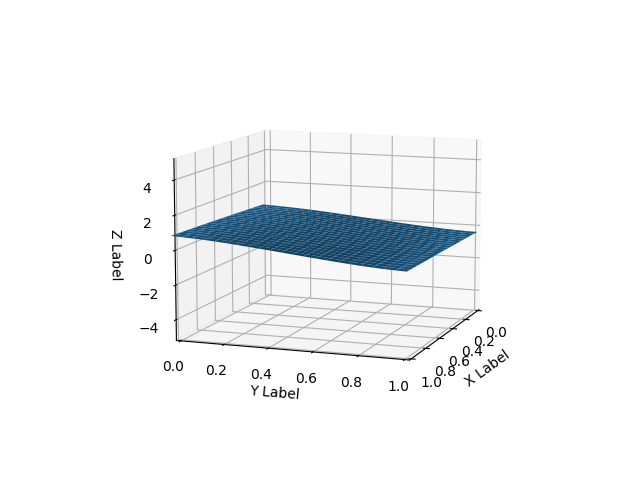
\includegraphics[width=\linewidth]{images/Interp_sol2.png}
		\end{figure}
	\end{columns}
\end{frame}


\begin{frame}{¿Porqué no para 3 partículas?}
	No se puedo aplicar en el caso que estudiamos ya que
	\begin{enumerate}
		\item Samplear en el interior del dominio en $\bbR^6$ no captura completamente las interacciones entre partículas.
		\item Los gradientes calculados con diferenciación automática no son confiables si no se aproximan directamente.
		\item En varias dimensiones el tiempo de parada en el método de interpolación no es practico de calcular.
		\item Las redes de cada método son bastante inestables en su entrenamiento.
	\end{enumerate}
Como alternativa podríamos usar la versión del teorema de Feynmann-Kac con caminos reflejados y parados en la condición de Dirichlet, modificando el costo terminal respectivo.
\end{frame}

\begin{frame}{Otra aplicación: Juegos de N agentes}
	Consideremos un juego con N agentes que se mueven según la dinámica \parencite{han_deep_2020}
	\begin{equation}
	\begin{split}
		&dX_t^{i}=\mu^{i}(t,\bfX_t,\bfAlp_t)dt+\sigma^{i}(t,\bfX_t,\bfAlp_t)dW_t^{i}+\sigma^{0}(t,\bfX_t,\bfAlp_t)dW_{t}^0\\
		&X_{0}^{i}=x_{0}^{i} \quad  i\in \mathcal{I},
	\end{split}
\end{equation}
En donde cada uno quiere minimizar su propio costo
\begin{equation}
	\label{eqn:individualCost}
	J^i(t,x,\bfAlp_t):=\expect*{\int_{t}^{T}f^i(t,\bfX_t,\bfAlp_t)dt +g^i(\bfX_T)\Big| X_t^i=x}.
\end{equation}
\end{frame}


\begin{frame}{Equilibrio de Nash}
	¿Qué debería hacer cada agente para optimizar su costo? Se vuelve un problema de teoría de juegos. Definimos un equilibrio de Nash para el problema como un conjunto de estrategias $\alpha$ tal que para todo $i\in\mathcal{I}$ y cualquier $\beta^i\in\mathcal{A}^i$ tenemos
	$$J^{i}(\bfAlp)\leq J^i(\alpha^{1,*},\ldots,\alpha^{i-1,*},\beta^i,\alpha^{i+1,*},\ldots ,\alpha^{N,*})$$
\end{frame}

\begin{frame}{Deep Fictitious Play}
	Para hallar este equilibrio vamos a optimizar cada agente conociendo lo mejor que harían los demás. Vamos a hacer esto iterativamente hasta llegar a una aproximación del equilibrio. En cada paso vamos a resolver la HJB
	\begin{equation}
		\dpartial{V^{i,m+1}}{t}-\lambda|\nabla_i V^{i,m+1}|^2+2\sqrt{\lambda}\bfAlp^{-i,m}\cdot \nabla_{-i} V^{i,m+1}+F(t,\bfX)+\nu\Delta V^{i,m+1}=0,
	\end{equation}
	Es la misma ecuación que resolvimos con Deep BSDE! 
	\begin{equation}
		\mu^i(t,\bfX)=2\sqrt{\lambda}\begin{bmatrix}
			\alpha^1(t,\bfX) \\
			\vdots\\
			\alpha^{i-1}(t,\bfX) \\
			0\\
			\alpha^{i+1}(t,\bfX)\\
			\vdots   \\
			\alpha^N(t,\bfX)
		\end{bmatrix}
		\quad\quad\quad
		\sigma^i(t,\bfX)=\sqrt{2\nu}\mathbb{I}_{2N\times 2N}
	\end{equation}
	y
	\begin{equation}
		f^i(t,\bfX,V(t,\bfX),\nabla V(t,\bfX))=-\lambda|\nabla_i V|^2+F^i(t,\bfX),
	\end{equation}
\end{frame}


\begin{frame}{Resultados}
	Después de 50 iteraciones del algoritmo obtenemos la siguiente trayectoria óptima
	\begin{figure}
		\centering
		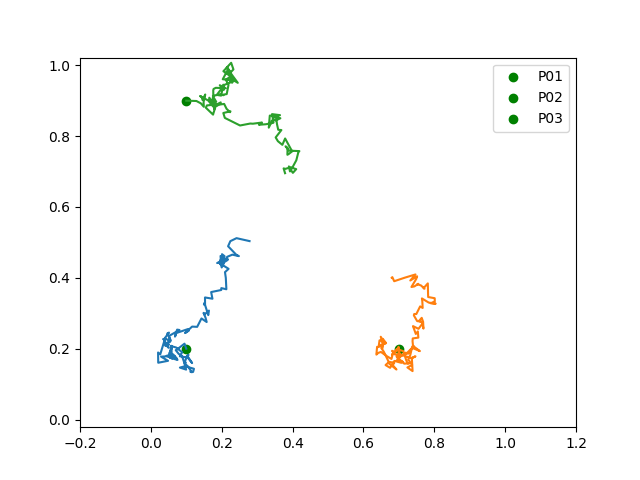
\includegraphics[height=6cm]{images/OptimalLQRDeepFictitus}
		\label{fig:optimallqrdeepfictitus}
	\end{figure}
\end{frame}

\begin{frame}{Conclusiones}
	\begin{itemize}
		\item Las redes neuronales permiten parametrizar funciones en espacios de alta dimensión. Esto los hace buenas candidatas para resolver ecuaciones diferenciales con estas características.
		\item Lamentablemente , estas no son muy estables ni robustas
	\end{itemize}
\end{frame}

\begin{frame}{Trabajo en curso}
	Nuestra idea original era usar estos métodos para resolver problemas de muchos agentes en dominios acotados para examinar las diferencias con soluciones de campo medio.\parencite{achdou_mean_2020}
	\begin{figure}
		\centering
		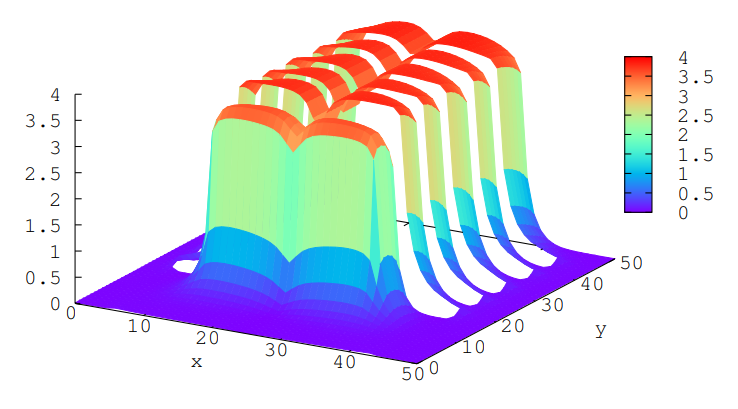
\includegraphics[width=0.7\linewidth]{images/achdou}
		\label{fig:achdou}
	\end{figure}

\end{frame}
\begin{frame}{Trabajo en curso}
	Y eventualmente estudiar numéricamente este cuadro
		\begin{figure}
		\centering
		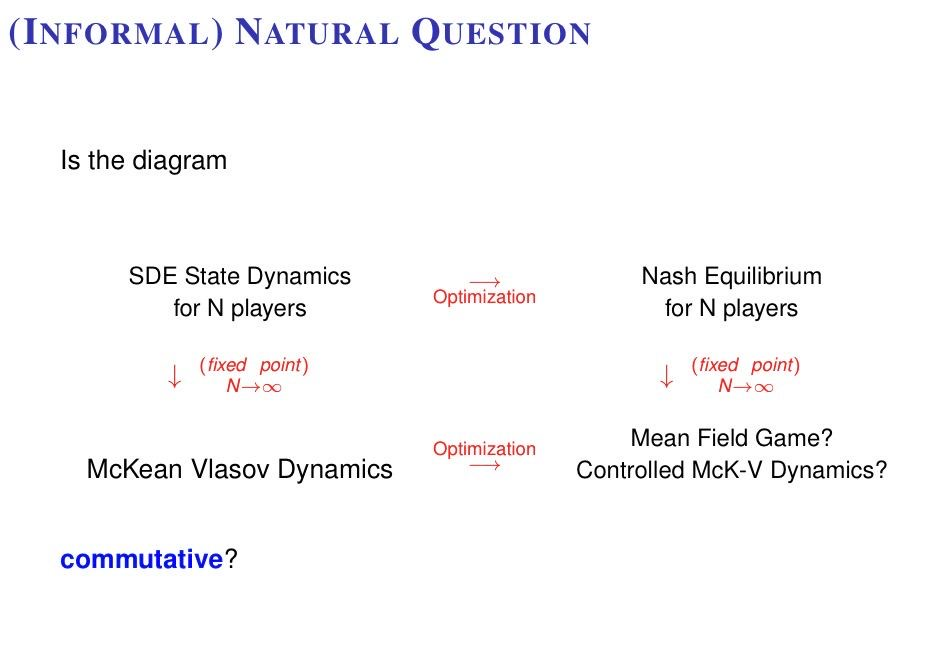
\includegraphics[width=0.7\linewidth]{images/cuadro}
		\label{fig:cuadro}
	\end{figure}
\end{frame}
%------------------------------------------------


%------------------------------------------------

\begin{frame}[allowframebreaks]{Referencias}
    % Beamer does not support BibTeX so references must be inserted manually as below
    
    \footnotesize{
\printbibliography
    }
\end{frame}

%------------------------------------------------

\begin{frame}
    \Huge{\centerline{\textbf{The End}}}
\end{frame}

%----------------------------------------------------------------------------------------
\end{document}